\documentclass[10pt,a4paper]{article}
\usepackage{a4wide,Z}
\newcommand{\ui}{\underline{i}}
\newcommand{\oi}{\overline{\imath}}


\usepackage{/usr/lib/R/share/texmf/Sweave}
\begin{document}


%\VignetteIndexEntry{strucchange: An R Package for Testing for Structural Change in Linear Regression Models}
%\VignetteDepends{strucchange}
%\VignetteKeywords{structural change, CUSUM, MOSUM, recursive estimates, moving estimates, monitoring, R, S}
%\VignettePackage{strucchange}

\title{\texttt{strucchange}: An \textsf{R}  Package for Testing for Structural
Change in Linear Regression Models}
\author{Achim Zeileis$^1$ \hspace{0.4cm} Friedrich Leisch$^1$ \hspace{0.4cm} Kurt Hornik$^1$ \hspace{0.4cm} Christian Kleiber$^2$\\
{\small $^1$ Institut f\"ur Statistik \& Wahrscheinlichkeitstheorie, Technische Universit\"at Wien,}\\
{\small $^2$ Institut f\"ur Wirtschafts- und Sozialstatistik, Universit\"at
Dortmund,}}
\date{}
\maketitle

\begin{abstract}
This introduction to the \textsf{R} package \texttt{strucchange} is a (slightly)
modified version of the paper of
\cite{sc:Zeileis+Leisch+Hornik:2002}, which
reviews tests for structural change in linear regression models from
the generalized fluctuation test framework as well as from the $F$ test (Chow
test) framework. It introduces a unified approach for implementing these tests
and presents how these ideas have been realized in {\tt strucchange}.
Enhancing the standard significance test approach the package contains
methods to fit, plot and test empirical fluctuation processes (like CUSUM, MOSUM
and estimates-based processes) and to compute, plot and test
sequences of $F$ statistics with the sup$F$, ave$F$ and exp$F$ test.
Thus, it makes powerful tools available to display information about
structural changes in regression relationships and to assess their significance.
Furthermore, it is described how incoming data can be monitored.
\end{abstract}

\noindent
{\bf Keywords:} structural change, CUSUM, MOSUM, recursive estimates, moving
estimates, monitoring, \textsf{R}, \textsf{S}.\\

\section{Introduction} \label{sec:intro}

The problem of detecting structural changes in linear regression relationships
has been an important topic in statistical and econometric research.
The most important classes of tests on structural change are the tests from the
generalized fluctuation test framework \citep{Z:Kuan+Hornik:1995} on the
one hand and tests based on $F$ statistics
\citep{Z:Hansen:1992,Z:Andrews:1993,Z:Andrews+Ploberger:1994} on the other.
The first class includes in particular the CUSUM and MOSUM tests and the
fluctuation test, while the Chow and the sup$F$ test belong to the latter.
A topic that gained more interest rather recently is to monitor structural
change, i.e., to start after a history phase (without structural changes) to
analyze new observations and to be able to detect a structural change as soon
after its occurrence as possible.\\

This paper concerns ideas and methods for implementing generalized fluctuation
tests as well as $F$ tests in a comprehensive and flexible way, that reflects
the common features of the testing procedures. It also offers facilities to
display the results in various ways.\\

This paper is organized as follows: In Section~\ref{sec:model} the standard
linear regression model upon which all tests are based will be described and the
testing problem will be specified. Section~\ref{sec:data} introduces a data set
which is also available in the package and which is used for the
examples in this paper. The following sections \ref{sec:fluctests},
\ref{sec:Ftests} and \ref{sec:monitor} will then explain the tests, how they are
implemented in {\tt strucchange} and give examples for each. Section
\ref{sec:fluctests} is concerned with computing empirical fluctuation processes,
with plotting them and the corresponding boundaries and finally with testing for
structural change based on these processes. Analogously,
Section~\ref{sec:Ftests} introduces the $F$ statistics and their plotting and
testing methods before Section~\ref{sec:monitor} extends the tools from
Section~\ref{sec:fluctests} for the monitoring case.


\section{The model} \label{sec:model}
Consider the standard linear regression model
\begin{equation} \label{model1} y_i = x_i^\top \beta_i + u_i
\qquad (i = 1, \dots, n), \end{equation}
where at time $i$, $y_i$ is the observation of the dependent
variable, $x_i = (1, x_{i2}, \dots, x_{ik})^\top$ is a $k \times 1$ vector of
observations of the independent variables, with the first component equal to
unity, $u_i$ are iid(0, $\sigma^2$), and $\beta_i$ is the $k \times 1$ vector of
regression coefficients. Tests on structural change are concerned with testing
the null hypothesis of ``no structural change''
\begin{equation} \label{null-hypothesis}
H_0: \quad \beta_i = \beta_0 \qquad (i = 1, \dots, n)
\end{equation}
against
the alternative that the coefficient vector varies over time, with
certain tests being more or less suitable (i.e., having good or poor power) for
certain patterns of deviation from the null hypothesis.\\

It is assumed
that the regressors are nonstochastic with $||x_i|| = O(1)$ and that
\begin{equation} \label{A5} \frac{1}{n} \sum_{i=1}^n x_i x_i^\top \quad
\longrightarrow \quad Q\end{equation}
for some finite regular matrix $Q$. These
are strict regularity conditions excluding trends in the data which are assumed
for simplicity. For some tests these assumptions can be
extended to dynamic models without changing the main properties of the tests;
but as these details are not part of the focus of this work they are omitted
here.\\

In what follows $\hat \beta^{(i, j)}$ is the ordinary least
squares (OLS) estimate of the regression coefficients based on the
observations $i+1, \dots, i+j$, and $\hat \beta^{(i)} = \hat \beta^{(0,i)}$ is
the OLS estimate based on all observations up to $i$. Hence $\hat \beta^{(n)}$
is the common OLS estimate in the linear regression model.
Similarly $X^{(i)}$ is the regressor matrix based on all observations up to $i$.
The OLS residuals
are denoted as $\hat u_i = y_i - x_i^\top \hat \beta^{(n)}$ with the
variance estimate $\hat{\sigma}^2 = \frac{1}{n-k}
\sum_{i=1}^n \hat u_i^2$. Another type of residuals that are often used in
tests on structural change are the recursive residuals \begin{equation}
\label{rr} \tilde u_i \; = \; \frac{y_i - x_i^\top \hat
\beta^{(i-1)}}{\sqrt{1+x_i^\top \left(X^{(i-1)^\top} X^{(i-1)} \right)^{-1}x_i}}
\qquad (i = k+1, \dots, n),\end{equation} which have zero mean and variance
$\sigma^2$ under the null hypothesis. The corresponding variance estimate is
$\tilde{\sigma}^2 = \frac{1}{n-k} \sum_{i=k+1}^n (\tilde u_i - \bar{ \tilde
u})^2$.

\section{The data} \label{sec:data}
The data used for examples throughout this paper are macroeconomic time
series from the USA. The data set contains the aggregated monthly personal
income and
personal consumption expenditures (in billion US dollars) between January 1959
and February 2001, which are seasonally adjusted at annual rates.
It was originally taken from \url{http://www.economagic.com/}, a web site for
economic times series. Both time series are depicted in Figure
\ref{fig:USIncExp}.

\setkeys{Gin}{width=0.6\textwidth}
\begin{figure}[htbp]
\begin{center}
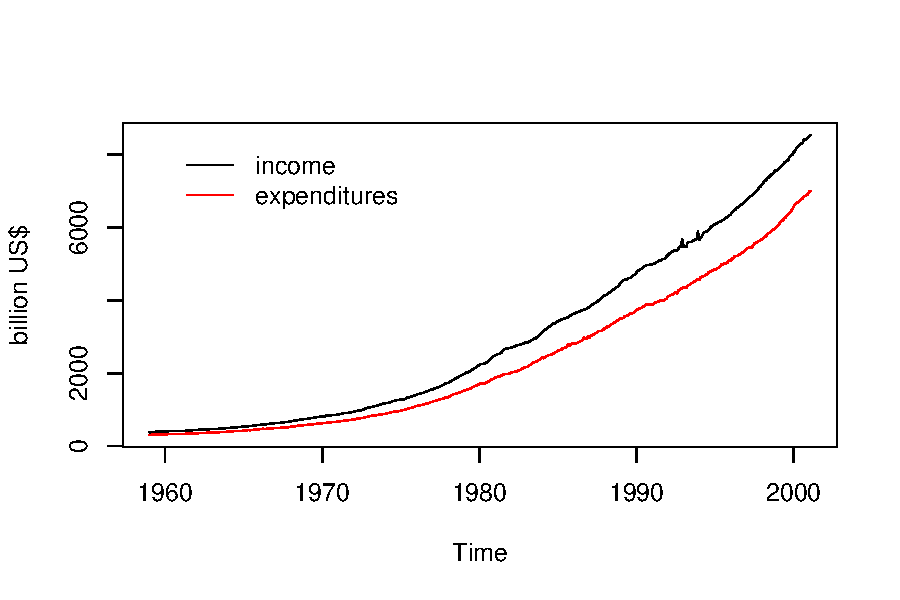
\includegraphics{strucchange-intro-data}
\caption{\label{fig:USIncExp} Personal income and personal consumption
expenditures in the US}
\end{center}
\end{figure}

The data is
available in the {\tt strucchange} package: it can be loaded and a
suitable subset chosen by
\begin{Schunk}
\begin{Sinput}
> library(strucchange)
> data(USIncExp)
> if (!"package:stats" %in% search()) library(ts)
> USIncExp2 <- window(USIncExp, start = c(1985, 12))
\end{Sinput}
\end{Schunk}

We use a simple error correction model (ECM) for the consumption function
similar to \cite{sc:Hansen:1992a}:
\begin{eqnarray} \label{ecm.model}
\Delta c_t & = & \beta_1 + \beta_2 \; e_{t-1} + \beta_3 \; \Delta i_t + u_t, \\
\label{coint.model} e_t & = & c_t - \alpha_1 - \alpha_2 \; i_t,
\end{eqnarray}
where $c_t$ is the consumption expenditure and $i_t$ the income. We estimate
the cointegration equation (\ref{coint.model}) by OLS and use the residuals
$\hat e_t$ as regressors in equation (\ref{ecm.model}), in which we will test
for structural change. Thus, the dependent variable is the increase in
expenditure and the regressors are the cointegration residuals and the
increments of income (and a constant).
To compute the cointegration residuals
and set up the model equation we need the following steps in \textsf{R}:
\begin{Schunk}
\begin{Sinput}
> coint.res <- residuals(lm(expenditure ~ income, data = USIncExp2))
> coint.res <- lag(ts(coint.res, start = c(1985, 12), freq = 12), 
+     k = -1)
> USIncExp2 <- cbind(USIncExp2, diff(USIncExp2), coint.res)
> USIncExp2 <- window(USIncExp2, start = c(1986, 1), end = c(2001, 
+     2))
> colnames(USIncExp2) <- c("income", "expenditure", "diff.income", 
+     "diff.expenditure", "coint.res")
> ecm.model <- diff.expenditure ~ coint.res + diff.income
\end{Sinput}
\end{Schunk}

Figure~\ref{fig:ts} shows the transformed time series necessary for estimation
of equation (\ref{ecm.model}).

\begin{figure}[htbp]
\begin{center}
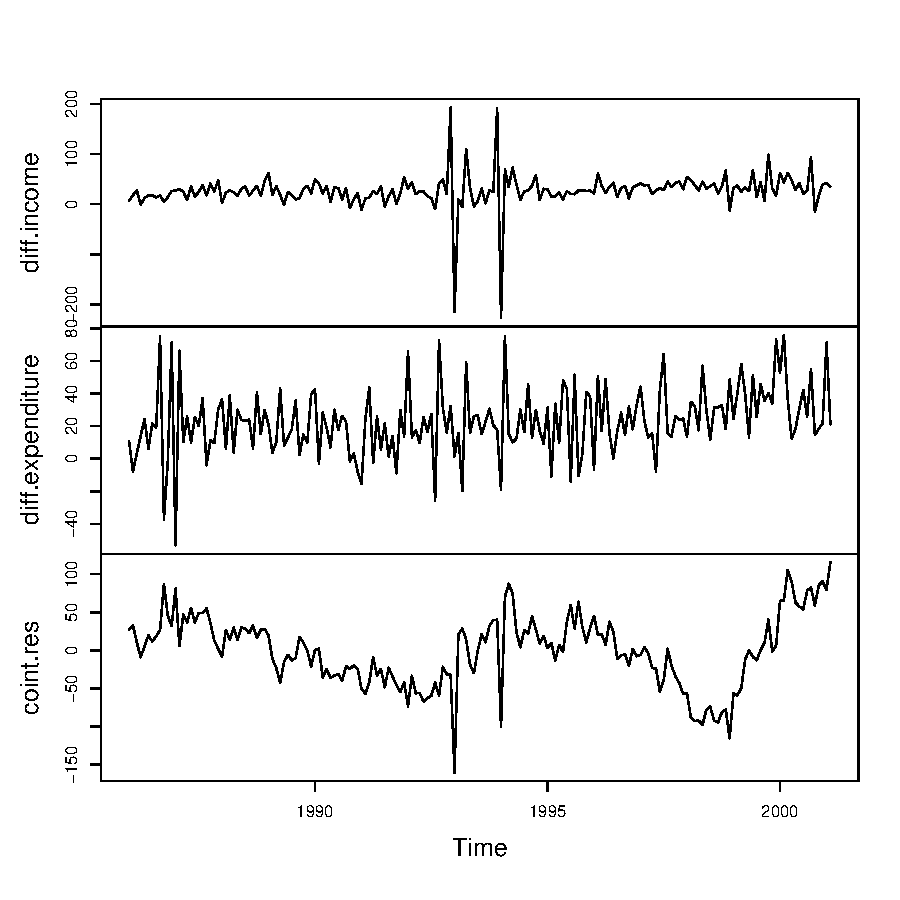
\includegraphics{strucchange-intro-ts-used}
\caption{\label{fig:ts} Time series used -- first differences and
cointegration residuals} \end{center}
\end{figure}


In the following sections we will apply the methods introduced to test for
structural change in this model.


\section{Generalized fluctuation tests} \label{sec:fluctests}

The generalized fluctuation tests fit a model to the given data and derive an
empirical process, that captures the fluctuation either in residuals or in
estimates. For these empirical processes the limiting processes are known, so
that boundaries can be computed, whose
crossing probability under the null hypothesis is $\alpha$. If the empirical
process path crosses these boundaries, the fluctuation is improbably large and
hence the null hypothesis should be rejected (at significance level $\alpha$).

\subsection{Empirical fluctuation processes: function \texttt{efp}}

Given a formula that describes a linear regression model to be tested the
function {\tt efp} creates an object of class {\tt "efp"} which contains
a fitted empirical fluctuation process of a specified type. The types
available will be described in detail in this section.\\

{\bf CUSUM processes}:
The first type of processes that can be computed are CUSUM processes, which
contain cumulative sums of standardized residuals.
\cite{Z:Brown+Durbin+Evans:1975} suggested to consider cumulative sums of
recursive residuals:
\begin{equation}\label{Rec-CUSUM} W_n(t) \; = \; \frac{1}{\tilde \sigma
\sqrt{\eta}}\sum_{i=k+1}^{k +\lfloor t\eta \rfloor} \tilde u_i \qquad (0
\le t \le 1),\end{equation}
where $\eta = n-k$ is the number of recursive residuals and $\lfloor t\eta
\rfloor$ is the integer part of $t\eta$.\\

Under the null hypothesis the limiting process for the empirical fluctuation
process $W_n(t)$ is the Standard Brownian Motion (or Wiener Process) $W(t)$.
More precisely the following functional central limit theorem (FCLT) holds:
\begin{equation}\label{lim(Rec-CUSUM)}  W_n \Longrightarrow W, \end{equation}
as $n \rightarrow \infty$, where $\Rightarrow$ denotes weak convergence
of the associated probability measures.\\

Under the alternative, if there is just a single structural change point $t_0$,
the recursive residuals will only have zero mean up to $t_0$. Hence the path of
the process should be close to 0 up to $t_0$ and leave its mean afterwards.
\cite{Z:Kraemer+Ploberger+Alt:1988}
show that the main properties of the CUSUM quantity remain the same even under 
weaker assumptions, in particular in dynamic models. Therefore {\tt efp} has the
logical argument {\tt dynamic}; if set to {\tt TRUE} the lagged observations
$y_{t-1}$ will be included as regressors.\\

\cite{Z:Ploberger+Kraemer:1992} suggested to
base a structural change test on cumulative sums of the common OLS residuals.
Thus, the OLS-CUSUM type empirical fluctuation process is defined by:
\begin{equation} \label{OLS-CUSUM} W_n^0(t)
\quad = \quad \frac{1}{\hat \sigma \sqrt{n}} \sum_{i=1}^{\lfloor nt \rfloor}
\hat u_i \qquad (0 \le t \le 1). \end{equation}
The limiting process for $W_n^0(t)$ is the standard Brownian bridge $W^0(t) =
W(t) - t W(1)$. It starts in 0 at $t = 0$ and it also returns to 0 for $t =
1$. Under a single structural shift alternative the path should have a peak
around $t_0$.\\

These processes are available in the function {\tt efp} by specifying the
argument {\tt type} to be either {\tt "Rec-CUSUM"} or {\tt "OLS-CUSUM"},
respectively.\\

{\bf MOSUM processes}:
Another possibility to detect a
structural change is to analyze moving sums of residuals (instead of using
cumulative sums of the same residuals).
The resulting empirical fluctuation process does then not contain the sum of all
residuals up to a certain time~$t$ but the sum of a fixed number of residuals in
a data window whose size is determined by the bandwidth parameter $h \in (0,1)$
and which is moved over the whole sample period. Hence the Recursive MOSUM
process is defined by
\begin{eqnarray} \label{Rec-MOSUM}
M_n(t | h) & = & \frac{1}{\tilde \sigma \sqrt{\eta}} \sum_{i =
k+\lfloor N_\eta t \rfloor +1}^{k+\lfloor N_\eta t \rfloor +\lfloor
\eta h \rfloor} \tilde u_i \qquad (0 \le t \le 1-h) \\
\label{Rec-MOSUM2}
& = &  W_n \left( \frac{ \lfloor N_\eta t \rfloor + \lfloor \eta
h\rfloor}{\eta} \right) - W_n \left( \frac{ \lfloor N_\eta t
\rfloor}{\eta} \right), \end{eqnarray}
where $N_\eta = (\eta - \lfloor \eta h \rfloor)/(1-h)$. Similarly the OLS-based
MOSUM process is defined by
\begin{eqnarray} \label{OLS-MOSUM}
M_n^0 (t | h) & = & \frac{1}{\hat \sigma \sqrt{n}} \left( \sum_{i =
\lfloor N_n t \rfloor +1}^{\lfloor N_n t \rfloor +\lfloor nh \rfloor} \hat u_i
\right) \qquad (0 \le t \le 1 - h) \\
\label{OLS-MOSUM2}
& = & W_n^0 \left( \frac{ \lfloor N_n t \rfloor + \lfloor n
h\rfloor}{n} \right) - W_n^0 \left( \frac{ \lfloor N_n t \rfloor}{n}
\right),
\end{eqnarray}
where $N_n = (n - \lfloor n h \rfloor)/(1-h)$. As the representations
(\ref{Rec-MOSUM2}) and (\ref{OLS-MOSUM2}) suggest, the limiting process
for the empirical MOSUM processes are the increments of a Brownian motion or a
Brownian bridge respectively. This is shown in detail in
 \cite{Z:Chu+Hornik+Kuan:1995}.\\

If again a single structural shift is assumed at $t_0$, then both MOSUM paths
should also have a strong shift around $t_0$.\\

The MOSUM processes will be computed if {\tt type} is set to {\tt "Rec-MOSUM"}
or {\tt "OLS-MOSUM"}, respectively.\\

{\bf Estimates-based processes}:
Instead of defining fluctuation processes on the basis of residuals they
can be equally well based on estimates of the unknown regression coefficients.
With the same ideas as for the residual-based CUSUM- and MOSUM-type processes
the $k \times 1$-vector $\beta$ is either estimated recursively with a growing
number of observations or with a moving data window of constant bandwidth $h$
and then compared to the estimates based on the whole sample.
The former idea leads to the fluctuation process  in the spirit of
\cite{Z:Ploberger+Kraemer+Kontrus:1989} which is defined by
\begin{equation}
\label{fluctuation} Y_n \left(t \right) = \frac{\sqrt{i}}{\hat \sigma
\sqrt{n}}  \left({X^{(i)}}^\top X^{(i)} \right)^{\frac{1}{2}} \left( \hat
\beta^{(i)} - \hat \beta^{(n)} \right), \end{equation}
where $i = \lfloor k + t(n-k) \rfloor$ with $t \in [0,1]$. And the latter gives
the moving estimates (ME) process introduced by \cite{Z:Chu+Hornik+Kuan:1995a}:
\begin{equation} \label{ME}
Z_n \left( \left. t \right| h \right) = \frac{\sqrt{\lfloor nh
\rfloor}}{\hat \sigma \sqrt{n}} \left({X^{(\lfloor nt \rfloor, \lfloor nh
 \rfloor)}}^\top X^{(\lfloor nt \rfloor,
\lfloor nh \rfloor)} \right)^{\frac{1}{2}} \left( \hat \beta^{(\lfloor nt
 \rfloor,\lfloor nh
\rfloor)} - \hat \beta^{(n)} \right), \end{equation}
where $0 \le t \le 1-h$.
Both are $k$-dimensional empirical processes. Thus, the limiting processes are a
$k$-dimensional Brownian Bridge or the increments thereof respectively. Instead
of rescaling the processes for each $i$ they can also be standardized by
$\left( {X^{(n)}}^\top X^{(n)} \right)^{\frac{1}{2}}$. This has the
advantage that it has to be calculated only once, but \cite{Z:Kuan+Chen:1994}
showed that if there are dependencies between the regressors the rescaling
improves the empirical size of the resulting test. Heuristically the rescaled
empirical fluctuation process ``looks'' more like its theoretic counterpart.\\

Under a single shift alternative the recursive estimates processes should
have a peak and the moving estimates process
should again have a shift close to the shift point $t_0$.\\

For {\tt type="fluctuation"} the function {\tt efp} returns the recursive
estimates process, whereas for {\tt "ME"} the moving estimates process is
returned.\\

All six processes may be fitted using the function {\tt efp}.
For our example we want to fit an OLS-based CUSUM process, and a moving
estimates (ME) process with bandwidth $h = 0.2$. The commands are simply
\begin{Schunk}
\begin{Sinput}
> ocus <- efp(ecm.model, type = "OLS-CUSUM", data = USIncExp2)
> me <- efp(ecm.model, type = "ME", data = USIncExp2, h = 0.2)
\end{Sinput}
\end{Schunk}
These return objects of class {\tt "efp"} which contain mainly the
empirical fluctuation processes and a few further attributes like the process
type. The process itself is of class {\tt "ts"} (the basic time series class in
\textsf{R}), which either preserves the time
properties of the dependent variable if this is a time series (like in our
example), or which is standardized to the interval $[0,1]$ (or a
subinterval). For the MOSUM and ME processes the centered interval $[h/2,
1-h/2]$ is chosen rather than $[0,1-h]$ as in (\ref{Rec-MOSUM}) and
(\ref{OLS-MOSUM}).\\

Any other process type introduced in this section can be fitted by setting the
{\tt type} argument. The fitted process can then be printed, plotted or tested
with the corresponding test on structural change. For the latter appropriate
boundaries are needed; the concept of boundaries for fluctuation processes is
explained in the next section.

\subsection{Boundaries and plotting}

The idea that is common to all generalized fluctuation tests is that the null
hypothesis of ``no structural change'' should be rejected when the fluctuation
of the empirical process $\mathit{efp}(t)$ gets improbably large compared to the
fluctuation of the limiting process. For the one-dimensional residual-based
processes this comparison is performed by some appropriate boundary $b(t)$, that
the limiting process just crosses with a given probability $\alpha$. Thus, if
$\mathit{efp}(t)$ crosses either $b(t)$ or $-b(t)$ for any $t$ then it has to be
concluded that the fluctuation is improbably large and the null hypothesis can
be rejected at confidence level $\alpha$. The procedure for the $k$-dimensional
estimates-based processes is similar, but instead of a boundary for the process
itself a boundary for $||\mathit{efp}_i(t)||$ is used,
where $||\cdot||$ is an appropriate functional which is applied component-wise.
We have implemented the functionals `max' and `range'. The null hypothesis is
rejected if $||\mathit{efp}_i(t)||$ gets larger than a constant $\lambda$, which
depends on the confidence level $\alpha$, for any $i = 1, \dots, k$.\\

The boundaries for the MOSUM processes are also constants, i.e., of form $b(t) =
\lambda$, which seems natural as the limiting processes are stationary. The
situation for the CUSUM processes is different though. Both limiting processes,
the Brownian motion and the Brownian bridge, respectively, are not stationary.
It would seem natural to use boundaries that are proportional to the standard
deviation function of the corresponding theoretic process, i.e.,
\begin{eqnarray}
\label{bound:Rec-CUS1} b(t) &=& \lambda \cdot \sqrt{t}\\
\label{bound:OLS-CUS1} b(t) &=& \lambda \cdot \sqrt{t(1-t)}
\end{eqnarray}
for the Recursive CUSUM and the OLS-based CUSUM path respectively,
where $\lambda$ determines the confidence level. But the
boundaries that are commonly used are linear, because a closed form solution for
the crossing probability is known. So the standard boundaries for the
two proccess are of type
\begin{eqnarray}
\label{bound:Rec-CUS} b(t) &=& \lambda \cdot (1+2t)\\
\label{bound:OLS-CUS} b(t) &=& \lambda.
\end{eqnarray}
They were chosen because they are tangential to the boundaries
(\ref{bound:Rec-CUS1}) and (\ref{bound:OLS-CUS1}) respectively in $t = 0.5$.
However, \cite{Zo:Zeileis:2000a} examined the properties of the alternative
boundaries (\ref{bound:Rec-CUS1}) and (\ref{bound:OLS-CUS1}) and showed that
the resulting OLS-based CUSUM test has better power
for structural changes early and late in the sample period.\\

Given a fitted empirical fluctuation process the boundaries can be
computed very easily using the function {\tt boundary}, which returns a time
series object with the same time properties as the given fluctuation process:
\begin{Schunk}
\begin{Sinput}
> bound.ocus <- boundary(ocus, alpha = 0.05)
\end{Sinput}
\end{Schunk}
It is also rather convenient to plot the process with its boundaries for some
confidence level $\alpha$ (by default 0.05) to see whether the path exceeds the
boundaries or not: This is demonstrated in Figure~\ref{fig:ocus}.

\begin{figure}[hbtp]
\begin{center}
\begin{Schunk}
\begin{Sinput}
> plot(ocus)
\end{Sinput}
\end{Schunk}
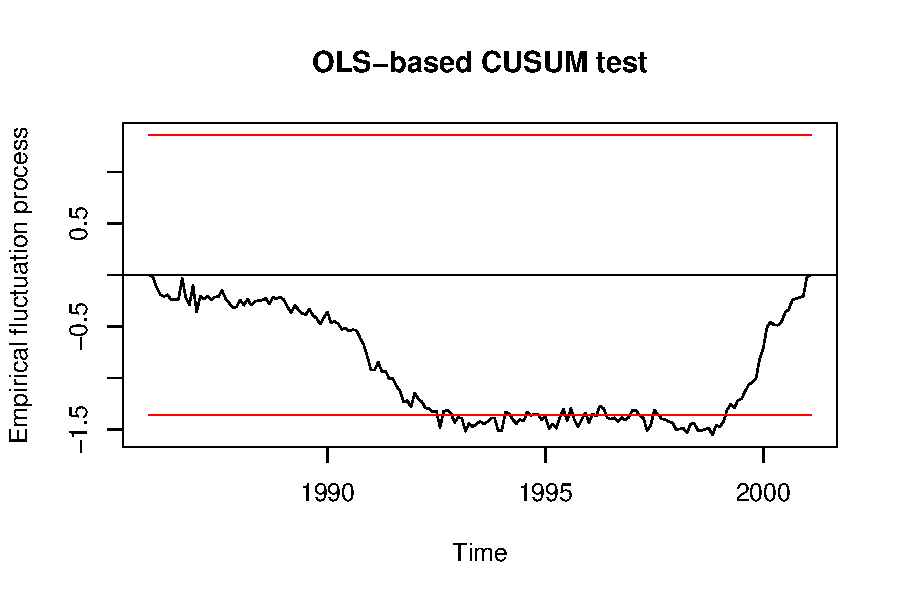
\includegraphics{strucchange-intro-OLS-CUSUM}
\caption{\label{fig:ocus} OLS-based CUSUM process}
\end{center}
\end{figure}

It can be seen that the OLS-based CUSUM process exceeds its boundary; hence
there is evidence for a structural change. Furthermore the process seems to
indicate two changes: one in the first half of the 1990s and another one at the
end of 1998.\\

It is also possible to suppress the boundaries and add them afterwards, e.g. in
another color
\begin{Schunk}
\begin{Sinput}
> plot(ocus, boundary = FALSE)
> lines(bound.ocus, col = 4)
> lines(-bound.ocus, col = 4)
\end{Sinput}
\end{Schunk}
For estimates-based processes it is only sensible to use time series plots if
the functional `max' is used because it is equivalent to rejecting the null
hypothesis when $\max_{i=1, \dots, k} ||\mathit{efp}(t)||$ gets large or when
$\max_t \max_{i=1, \dots, k} \mathit{efp}_i(t)$ gets large. This again is
equivalent to any one of the (one-dimensinal) processes $\mathit{efp}_i(t)$ for
$i = 1, \dots, k$ exceeding the boundary. The $k$-dimensional process can also
be plotted by specifying the parameter {\tt functional} (which defaults to {\tt
"max"}) as {\tt NULL}:

\begin{figure}[h]
\begin{center}
\begin{Schunk}
\begin{Sinput}
> plot(me, functional = NULL)
\end{Sinput}
\end{Schunk}
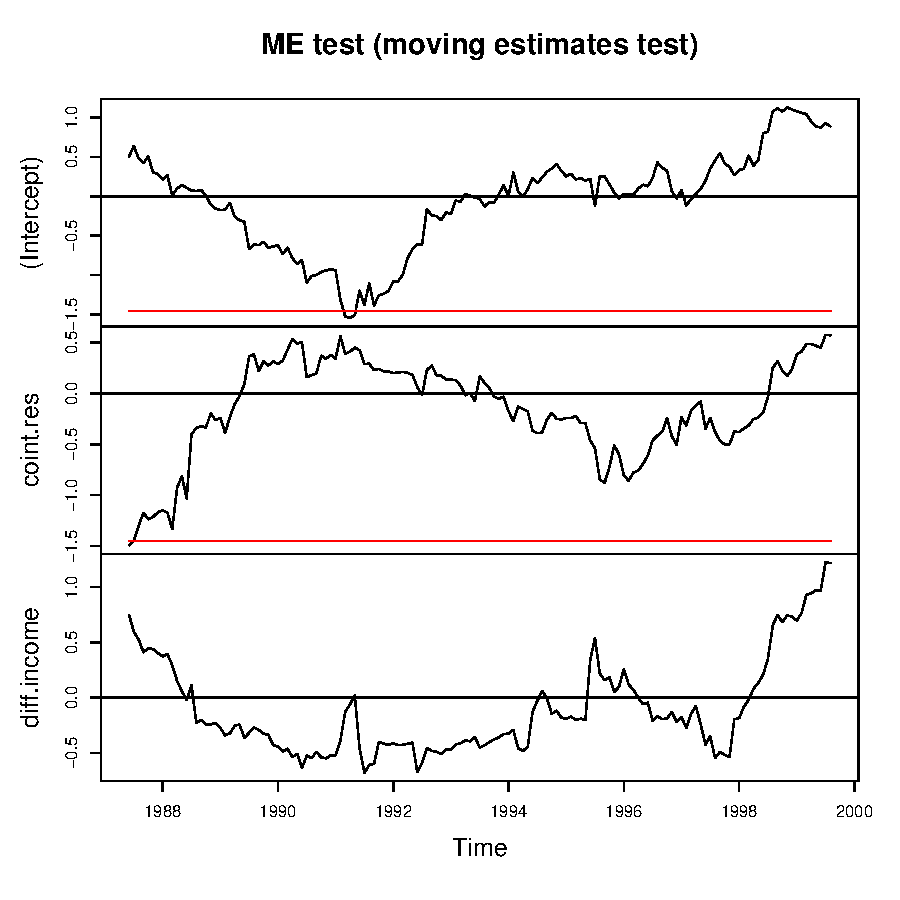
\includegraphics{strucchange-intro-ME-null}
\caption{\label{fig:me-null} 3-dimensional moving estimates process}
\end{center}
\end{figure}

The output from \textsf{R} can be seen in Figure~\ref{fig:me-null}, where the
three parts of the plot
show the processes that correspond to the estimate of the
regression coefficients of the intercept, the cointegration residuals and the
increments of income, respectively. All three paths show two shifts: the first
shift starts at the beginning of the sample period and ends in about 1991 and
the second shift occurs at the very end of the sample period. The shift that
causes the significance seems to be the strong first shift in the process for
the intercept and the cointegration residuals, because these cross their
boundaries. Thus, the ME test leads to similar results as the
OLS-based CUSUM test, but provides a little more information about the nature of
the structural change.

\subsection{Significance testing with empirical fluctuation processes}

Although calculating and plotting the empiricial fluctuation process with its
boundaries provides and visualizes most of the information, it might still be
necessary or desirable to carry out a traditional significance test. This can be
done easily with the function {\tt sctest} (\underline{s}tructural
\underline{c}hange \underline{test}) which returns an object of class {\tt
"htest"} (\textsf{R}'s standard class for statistical test results) containing
in particular the test statistic and the corresponding $p$ value. The test
statistics reflect what was described by the crossing of boundaries in the
previous section. Hence the test statistic is $S_r$ from (\ref{statr}) for the
residual-based processes and $S_e$ from (\ref{state}) for the estimates-based
processes: \begin{eqnarray} \label{statr} S_r & = & \max_t
\frac{\mathit{efp}(t)}{f(t)},\\ \label{state} S_e & = & \max
||\mathit{efp}(t)||, \end{eqnarray}
where $f(t)$ depends on the shape of the boundary, i.e.,
$b(t) = \lambda \cdot f(t)$. For most boundaries is $f(t) \equiv 1$, but the
linear boundary for the Recursive CUSUM test for example has shape $f(t) = 1 + 
2t$.\\

It is either possible to supply {\tt sctest} with a fitted
empirical fluctuation process or with a formula describing the model that should
be tested. Thus, the commands
\begin{Schunk}
\begin{Sinput}
> sctest(ocus)
\end{Sinput}
\end{Schunk}
and
\begin{Schunk}
\begin{Sinput}
> sctest(ecm.model, type = "OLS-CUSUM", data = USIncExp2)
\end{Sinput}
\begin{Soutput}
	OLS-based CUSUM test

data:  ecm.model 
S0 = 1.5511, p-value = 0.01626
\end{Soutput}
\end{Schunk}
lead to equivalent results.
{\tt sctest} is a generic function which has methods not only for
fluctuation tests, but all
structural change tests (on historic data) introduced in this paper including
the $F$ tests described in the next section.


\section{$F$ tests} \label{sec:Ftests}

A rather different approach to investigate whether the null hypothesis
of ``no structural change'' holds, is to use $F$ test statistics. An important
difference is that the alternative is specified: whereas the generalized
fluctuation tests are suitable for various patterns of structural changes, the
$F$ tests are designed to test against a single shift alternative. Thus, the
alternative can be formulated on the basis of the model (\ref{model1})
\begin{equation} \label{H1}
\beta_i = \left\{ \begin{array}{l} \beta_A \quad (1 \le i \le i_0) \\
\beta_B \quad (i_0 < i \le n) \end{array} \right.,
\end{equation}
where $i_0$ is some change point in the interval $(k, n-k)$. \cite{Z:Chow:1960}
was the first to suggest such a test on structural change for the case where the
(potential) change point $i_0$ is known.
He proposed to fit two separate regressions for the two subsamples defined by
$i_0$ and to reject whenever
\begin{equation} \label{Fstat}
F_{i_0} \; = \; \frac{{\hat u}^\top {\hat u} - {\hat e}^\top {\hat
e}}{{\hat e}^\top {\hat e}/(n-2k)}.
\end{equation}
is too large, where $\hat e = (\hat u_A, \hat u_B)^\top$ are the residuals from
the full model, where the coefficients in the subsamples are estimated
separately, and $\hat u$ are the residuals from the restricted model, where the
parameters are just fitted once for all observations. The test statistic
$F_{i_0}$ has an asymptotic $\chi^2$ distribution with $k$ degrees of freedom 
and (under the assumption of normality) $F_{i_0}/k$ has an exact $F$
distribution with $k$ and $n-2k$ degrees of freedom. The major drawback of this
``Chow test'' is that the change point has to be known in advance, but there are
tests based upon $F$ statistics (Chow statistics), that do not require a
specification of a particular change point and which will be introduced in the
following sections.

\subsection{$F$ statistics: function \texttt{Fstats}}

A natural idea to extend the ideas from the Chow test is to calculate the $F$
statistics for all potential change points or for all potential change points in
an interval $[\ui, \oi]$ and to reject if any of those statistics get too large.
Therefore the first step is to compute the $F$ statistics $F_i$ for $k < \ui \le
i \le \oi < n-k$, which can be easily done using the function {\tt Fstats}.
Again the model to be tested is specified by a formula interface and the
parameters $\ui$ and $\oi$ are respresented by {\tt from} and {\tt to},
respectively. Alternatively to indices of observations these two parameters can 
also be specified by fractions of the sample; the default is to take {\tt from =
0.15} and implicitly {\tt to = 0.85}. To compute the $F$ test statistics for all
potential change points between January 1990 and June 1999 the appropriate
command would be:
\begin{Schunk}
\begin{Sinput}
> fs <- Fstats(ecm.model, from = c(1990, 1), to = c(1999, 6), data = USIncExp2)
\end{Sinput}
\end{Schunk}
This returns an object of class {\tt "Fstats"} which mainly contains a time
series of $F$ statistics. Analogously to the empiricial fluctuation processes
these objects can be printed, plotted and tested.

\subsection{Boundaries and plotting}

The computation of boundaries and plotting of $F$ statistics is rather similar
to that of empirical fluctuation processes introduced in the previous section.
Under the null hypthesis of no structural change boundaries can be computed
such that the asymptotic probability that the supremum (or the mean) of the
statistics $F_i$ (for $\ui \le i \le \oi$) exceeds this boundary is $\alpha$.
So the following command
\begin{figure}[htbp]
\begin{center}
\begin{Schunk}
\begin{Sinput}
> plot(fs)
\end{Sinput}
\end{Schunk}
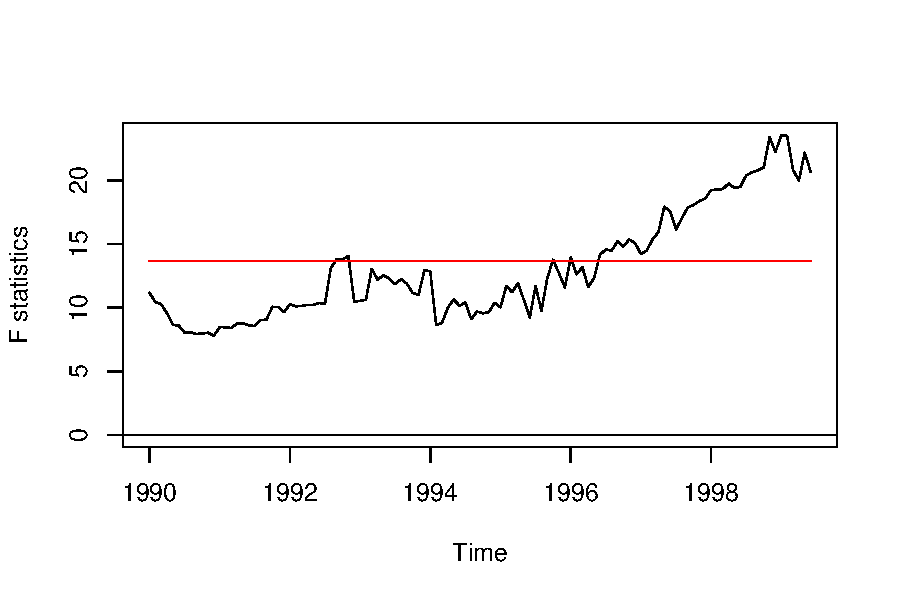
\includegraphics{strucchange-intro-Fstats-plot}
\caption{\label{fig:Fstats} $F$ statistics}
\end{center}
\end{figure}
plots the process of $F$ statistics with its boundary;
the output can be seen in
Figure~\ref{fig:Fstats}. As the $F$ statistics cross their boundary, there is
evidence for a structural change (at the level $\alpha = 0.05$). The process
has a clear peak in 1998, which mirrors
the results from the analysis by empirical fluctuation processes and tests,
respectively, that also indicated a break in the late 1990s.\\

It is also possible to plot the $p$ values instead of
the $F$ statistics themselves by
\begin{Schunk}
\begin{Sinput}
> plot(fs, pval = TRUE)
\end{Sinput}
\end{Schunk}
which leads to equivalent results. Furthermore it is also possible to set up
the boundaries for the average instead of the supremum by:
\begin{Schunk}
\begin{Sinput}
> plot(fs, aveF = TRUE)
\end{Sinput}
\end{Schunk}
In this case another dashed line for the observed mean of the $F$ statistics
will be drawn.

\subsection{Significance testing with $F$ statistics}

As already indicated in the previous section, there is more than one
possibility to aggregate the series of $F$ statistics into a test statistic.
\cite{Z:Andrews:1993} and \cite{Z:Andrews+Ploberger:1994} respectively suggested
three different test statistics and examined their asymptotic distribution:
\begin{eqnarray}
\label{supF} \mbox{\textnormal{sup}}F & = & \sup_{\ui\le i \le \oi} F_i, \\
\label{aveF} \mbox{\textnormal{ave}}F & = & \frac{1}{\oi - \ui+ 1}
\sum_{i = \ui}^{\oi} F_i, \\
\label{expF} \mbox{\textnormal{exp}}F & = & \log \left( \frac{1}{\oi - \ui+
1} \sum_{i = \ui}^{\oi} \exp ( 0.5 \cdot F_i) \right).
\end{eqnarray}
The sup$F$ statistic in (\ref{supF}) and the ave$F$ statistic from
(\ref{aveF}) respectively reflect the testing procedures that have been
described above. Either the null hypothesis is rejected when the maximal or the
mean $F$ statistic gets too large. A third possibility is to reject when the
exp$F$ statistic from (\ref{expF}) gets too large. The ave$F$ and exp$F$ test
have certain optimality properties \citep{Z:Andrews+Ploberger:1994}.
The tests can be carried out
in the same way as the fluctuation tests: either by supplying the fitted {\tt
Fstats} object or by a formula that describes the model to be tested. Hence the
commands
\begin{Schunk}
\begin{Sinput}
> sctest(fs, type = "expF")
\end{Sinput}
\end{Schunk}
and
\begin{Schunk}
\begin{Sinput}
> sctest(ecm.model, type = "expF", from = 49, to = 162, data = USIncExp2)
\end{Sinput}
\begin{Soutput}
	expF test

data:  ecm.model 
exp.F = 8.9955, p-value = 0.001311
\end{Soutput}
\end{Schunk}
lead to equivalent output.

The $p$ values are computed based on \cite{Z:Hansen:1997}.\footnote{The authors
thank Bruce Hansen, who wrote the original code for computing $p$ values for $F$
statistics in \textsf{GAUSS}, for putting his code at disposal for porting to
\textsf{R}.}


\section{Monitoring with the generalized fluctuation test}
\label{sec:monitor}

In the previous sections we were concerned with the retrospective detection
of structural changes in \emph{given} data sets. Over the last years
several structural change tests have been extended to monitoring
of linear regression models where new data arrive over time
\citep{Z:Chu+Stinchcombe+White:1996,Z:Leisch+Hornik+Kuan:2000}. Such
forward looking tests are closely related to sequential tests. When
new observations arrive, estimates are computed sequentially from all
available data (historical sample plus newly arrived data) and compared
to the estimate based only on the historical sample. As in the
retrospective case, the hypothesis of no structural change is
rejected if the difference between these two estimates gets too large.

The standard linear regression model~(\ref{model1}) is generalized to
\begin{equation}
  y_i = x_i^\top \beta_i + u_i
  \qquad (i = 1, \dots, n, n+1, \ldots),
\end{equation}
i.e., we expect new observations to arrive after time $n$ (when the
monitoring begins). The sample $\{(x_1,y_1),\ldots,(x_n,y_n)\}$ will
be called the \emph{historic sample}, the corresponding time period
$1,\ldots,n$ the \emph{history period}.

Currently monitoring has only been developed for recursive
\citep{Z:Chu+Stinchcombe+White:1996} and moving
\citep{Z:Leisch+Hornik+Kuan:2000} estimates tests. The respective
limiting processes are---as in the retrospective case---the Brownian
Bridge and increments of the Brownian Bridge. The empirical
processes are rescaled to map the history period to the interval [0,1]
of the Brownian Bridge. For recursive estimates there exists a closed
form solution for boundary functions, such that the limiting Brownian
Bridge stays within the boundaries on the interval $(1,\infty)$ with
probability $1-\alpha$. Note that the monitoring period consisting of
all data arriving after the history period corresponds to the Brownian
Bridge after time 1. For moving estimates, only the growth rate of the
boundaries can be derived analytically and critical values have to be
simulated.

Consider that we want to monitor our ECM during the
1990s for structural change, using years 1986--1989 as the history
period. First we cut the historic sample from the complete data set
and create an object of class \texttt{"mefp"}:
\begin{Schunk}
\begin{Sinput}
> USIncExp3 <- window(USIncExp2, start = c(1986, 1), end = c(1989, 
+     12))
> me.mefp <- mefp(ecm.model, type = "ME", data = USIncExp3, alpha = 0.05)
\end{Sinput}
\end{Schunk}
Because monitoring is a sequential test procedure, the
significance level has to be specified \emph{in advance}, i.e., when
the object of class \texttt{"mefp"} is created. The \texttt{"mefp"}
object can now be monitored repeatedly for structural changes.

Let us assume we get new observations for the year 1990. Calling function
\texttt{monitor} on \texttt{me.mefp} automatically updates our
monitoring object for the new observations and runs a sequential test
for structural change on each new observation (no structural break is
detected in 1990):
\begin{Schunk}
\begin{Sinput}
> USIncExp3 <- window(USIncExp2, start = c(1986, 1), end = c(1990, 
+     12))
> me.mefp <- monitor(me.mefp)
\end{Sinput}
\end{Schunk}
Then new data for the years 1991--2001 arrive and we repeat the
monitoring:
\begin{Schunk}
\begin{Sinput}
> USIncExp3 <- window(USIncExp2, start = c(1986, 1))
> me.mefp <- monitor(me.mefp)
\end{Sinput}
\begin{Soutput}
Break detected at observation # 72 
\end{Soutput}
\begin{Sinput}
> me.mefp
\end{Sinput}
\begin{Soutput}
Monitoring with ME test (moving estimates test) 

Initial call:
  mefp.formula(formula = ecm.model, type = "ME", data = USIncExp3,      alpha = 0.05) 

Last call:
  monitor(obj = me.mefp) 

Significance level   :  0.05 
Critical value       :  3.109524 
History size         :  48 
Last point evaluated :  182 
Structural break at  :  72 

Parameter estimate on history :
(Intercept)   coint.res diff.income 
 18.9299679  -0.3893141   0.3156597 
Last parameter estimate :
(Intercept)   coint.res diff.income 
27.94869106  0.00983451  0.13314662 
\end{Soutput}
\end{Schunk}
The software informs us that a structural break has been detected at
observation \#72, which corresponds to December 1991. Boundary and
plotting methods for \texttt{"mefp"} objects work (almost) exactly as
their \texttt{"efp"} counterparts, only the significance level
\texttt{alpha} cannot be specified, because it is specified when the
\texttt{"mefp"} object is created. The output of
\texttt{plot(me.mefp)} can be seen in Figure~\ref{fig:monitor}.

\begin{figure}[htbp]
\begin{center}
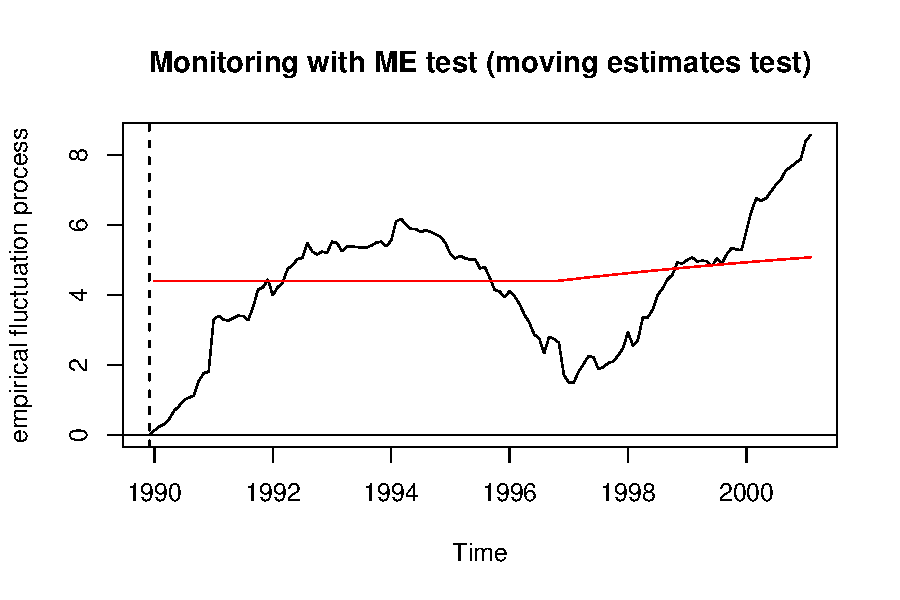
\includegraphics{strucchange-intro-monitor-plot}
\caption{\label{fig:monitor} Monitoring structural change with bandwidth $h=1$}
\end{center}
\end{figure}

Instead of creating an {\tt "mefp"} object using the formula interface like
above, it could also be done re-using an existing \texttt{"efp"} object, e.g.:
\begin{Schunk}
\begin{Sinput}
> USIncExp3 <- window(USIncExp2, start = c(1986, 1), end = c(1989, 
+     12))
> me.efp <- efp(ecm.model, type = "ME", data = USIncExp3, h = 0.5)
> me.mefp <- mefp(me.efp, alpha = 0.05)
\end{Sinput}
\end{Schunk}
If now again the new observations up to February 2001 arrive, we can monitor
the data
\begin{Schunk}
\begin{Sinput}
> USIncExp3 <- window(USIncExp2, start = c(1986, 1))
> me.mefp <- monitor(me.mefp)
\end{Sinput}
\begin{Soutput}
Break detected at observation # 70 
\end{Soutput}
\end{Schunk}
and discover the structural change even two observations earlier as we used
the bandwidth {\tt h=0.5} instead of {\tt h=1}. Due to this we have not one
history estimate that is being compared with the new moving estimates, but we
have a history process, which can be seen on the left in
Figure~\ref{fig:monitor2}. This plot can simply be generated by
\texttt{plot(me.mefp)}.

\begin{figure}[htbp]
\begin{center}
\includegraphics{strucchange-intro-monitor-plot2}
\caption{\label{fig:monitor2} Monitoring structural change with
bandwidth $h=0.5$} \end{center}
\end{figure}

The results of the monitoring emphasize the results of the historic tests: the
moving estimates process has two strong shifts, the first around 1992 and the
second around 1998.

\section{Conclusions} \label{sec:conclusions}

In this paper, we have described the {\tt strucchange} package that implements
methods for testing for structural change in linear regression relationships.
It provides a unified framework for displaying information
about structural changes flexibly and for assessing their significance
according to various tests.\\

Containing tests from the generalized fluctuation test framework as well as
tests based on $F$ statistics (Chow test ststistics) the package extends
standard significance testing procedures: There are methods for fitting
empirical fluctuation processes (CUSUM, MOSUM and estimates-based
processes), computing an appropriate boundary, plotting these results and
finally carrying out a formal significance test. Analogously a sequence of $F$
statistics with the corresponding boundary can be computed, plotted and tested.
Finally the methods for estimates-based fluctuation processes have extensions to
monitor incoming data.


\section*{Acknowledgements}

This research of Achim Zeileis, Friedrich Leisch and Kurt Hornik was supported
by the Austrian Science Foundation (FWF) under grant SFB\#010 (`Adaptive
Information Systems and Modeling in Economics and Management Science').\\
The work of Christian Kleiber was supported by the
Deutsche Forschungsgemeinschaft, Sonderforschungsbereich 475.

\newpage

\bibliography{Z,Zo,sc}
\bibliographystyle{abbrvnat}

\newpage
\begin{appendix}
\section{Implementation details for $p$ values}

An important and useful tool concerning significance tests are $p$ values,
especially for application in a software package. Their implementation is
therefore crucial and in this section we will give more detail about the
implementation in the {\tt strucchange} package.\\

For the CUSUM tests with linear boundaries there are rather good
approximations to the asymptotic $p$ value functions given in
\cite{Zo:Zeileis:2000a}. For the recursive estimates fluctuation test
there is a series expansion, which is evaluated for the first hundred terms. For
all other tests from the generalized fluctuation test framework the $p$ values
are computed by linear interpolation from tabulated critical values. For the
Recursive CUSUM test with alternative boundaries $p$ values from the interval
$[0.001, 1]$ and $[0.001, 0.999]$ for the OLS-based version respectively are
approximated from tables given in \cite{Zo:Zeileis:2000}. The critical values
for the Recursive MOSUM test for levels in $[0.01, 0.2]$ are taken from
\cite{Z:Chu+Hornik+Kuan:1995}, while the critical values for the levels
in $[0.01, 0.1]$ for the OLS-based MOSUM and the ME test are given in
\cite{Z:Chu+Hornik+Kuan:1995a}; the parameter $h$ is in both cases interpolated
for values in $[0.05, 0.5]$.\\

The $p$ values for the sup$F$, ave$F$ and exp$F$ test are approximated based on
\cite{Z:Hansen:1997}, who also wrote the original code in \textsf{GAUSS}, which
we merely ported to \textsf{R}. The computation uses tabulated simulated
regression coefficients.

\end{appendix}

\end{document}
